\section{Kalibrierung der Brille}
Im folgenden Kapitel soll geklärt werden, warum eine Durchsichtbrille kalibriert werden sollte. Hierbei werden folgende Fragen beantwortet: Wie ist die Brille zu kalibrieren, sodass eine Darstellung der erweiterten Realität problemlos möglich ist? Welche Konfigurationen sollen individuell vorgenommen werden, damit nicht jeder Nutzer \" schielen" muss, sobald er durch die 3D-Brille schaut? Wie wird die Wahrnehmung der 3D-Objekte mithilfe der Brillendisplays überhaupt möglich?

\subsection{Workflow}
Um eine 3D-Durchsichtbrille so zu kalibrieren, dass auf dieser reale und authentisch wirkende 3D Welten angezeigt werden können, muss diese präzise kalibriert sein. Wird ein 3D Film angesehen, ist die exakte Kalibrierung nicht entscheidend, soll jedoch eine Simulation einer AR-Welt in korrekten Dimensionen wahrgenommen werden, wird die Kalibrierung unabdingbar. Dies ist der Fall, wenn die Durchsichtbrille für diverse Szenarien im Kontext der kognitiven Automobile verwendet wird. Hierzu gehören Anwendungen, bei den z.B. Fußgänger simuliert werden um menschliche Fahrerinteraktionen zu messen und als Lerndaten zu akquirieren. Eine weitere Anwendung wäre die Visualisierung von simulierten Daten des Fahrzeuges für den Fahrer, damit dieser in einer simulierten Welt beurteilen kann, wie gut das kognitive Automobil sich einer Situation, z.B. beim Einparken verhält. Ebenfalls wird es möglich, mit einer kalibrierten Brille simulierte neue Bedienelemente eines Autos zu testen und deren Wirkung auf den Fahrer auszuprobieren.

Hierzu werden die Parameter benötigt, mit denen die Bilder für ein solch akkurates Stereoscopic-3D benötigt werden. Zu diesen Parametern zählen die Position der Augen, die Position der Bildschirme in den Brillengläsern und die Öffnungswinkel, mit denen ein einzelnes Individuum durch eine spezifische Brille sehen kann. Um diese Parameter zu bestimmen wurde ein interaktives Kalibrierungsverfahren ausgewählt, da es wichtig ist, dass die Kalibrierung komfortabel und ohne externe Gerätschaften von statten geht, da es für jeden Benutzter nötig ist, die Brille individuell zu kalibrieren. Das Minimum an benötigten Punkten um die Position eines Auges zu bestimmen sind zwei Geraden, also zwei Punkte auf einer Sichtlinie je Geraden. Um die Daten präziser zu machen können mehrere Geraden verwendet werden, die dann einen genaueren Schnittpunkt ermöglichen, es sollen aber immer nur 2 Punkte je Gerade verwendet werden, da bei dem Aufeinanderlegen von 3 Punkten für den Benutzer unangenehmen Haltungen während der Kalibrierung resultieren.

Der erste Ansatz war es einen Punkt im Auto zu verwenden, der in seiner Position bekannt ist und durch Bildverarbeitung erkannt werden kann und n Punkte auf der Brille. Hierbei hat sich jedoch herausgestellt, dass der Abstand der einzelnen Schnittlinien in einem sehr kleinen Winkels von statten geht und somit fehleranfällig ist. Der zweite Ansatz verwendet den Bildschirm, der im Auto verbaut ist und die Brillengläser. Hiermit sind beidseitig die Punkte variabel und können somit so gewählt werden, dass sich Messfehler nicht so gravierend auswirken wie im vorherigen Ansatz. Des Weiteren ist das Verfahren erweiterbar auf eine Onlinebewertung während der Kalibrierung, so dass über ein Algorithmus passende Punkte ausgewählt werden können, um die Kalibrierung zu optimieren.

Im Ablauf werden nun also Punkte auf dem Brillenglas angezeigt, die der Benutzer per Klick auf die Stelle auf dem Bildschirm markiert, so dass sie für ihn übereinander liegen. Somit konnte ein idealer Kompromiss zwischen Benutzerfreundlichkeit und der Akquisition von geeigneten Linienpaaren gefunden werden.

Nach dem Kalibrierungsprozess für jedes Auge können die benötigten Parameter berechnet werden.


\subsection{Bestimmung von Punktepaaren}
\label{chap:punktepaare}
\subsubsection{Konzept}
Um nun also Punktepaare für die Kalibrierung aufzeichnen zu können, ist die Grafikausgabe der Software nötig. Hierzu wurden zwei Anwendungen als ROS Nodes implementiert. Die Nodes werden mittels der Frameworks SDL und Qt umgesetzt.
\subsubsection{Anzeige auf der Brille}
Eine Vollbildanzeige mit fester Auflösung der nativen Auflösung der Brillenanzeige wird mittels SDL implementiert. Diese Anwendung erkennt automatisch die Brille als zweiten Bildschirm und wählt diesen für die Anzeige aus. Ansonsten ermöglicht die Anwendung es, einen Punkt an eine per ROS-Paket vorgegebene Position anzuzeigen.
Screenshot
\subsubsection{Anzeige auf dem Bildschirm}
Um auf den im Auto integrierten Bildschirm eine Anzeige durchzuführen, wurde eine Oberfläche (siehe Abbildung \ref{fig:fensteranwendung}) mit Qt implementiert. Diese enthält die für die Bildverarbeitung nötigen Marker (siehe Kapitel \ref{ssection:alva}) und nimmt die Klickpositionen vom Nutzer entgegen. Die ermittelte Klickposition wird als ROS-Messages versendet.
\begin{figure}[h]
   \centering
   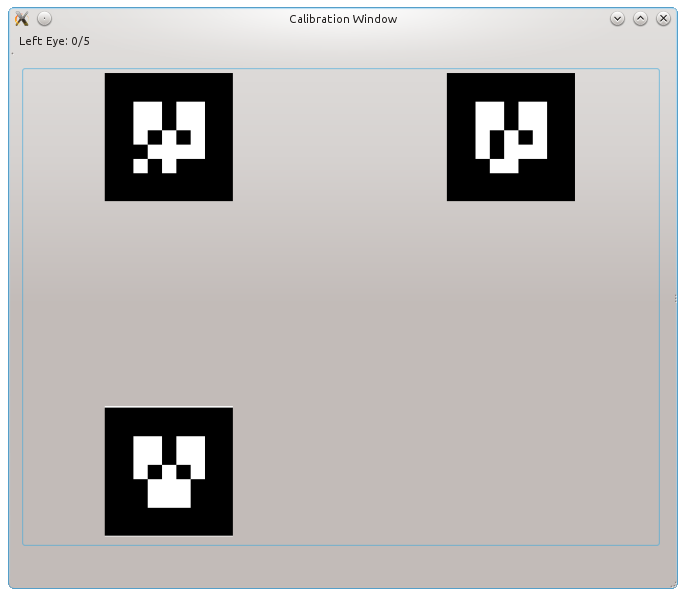
\includegraphics[width=0.45\textwidth]{bildschirm_anwendung}
   \caption{Oberfläche für den OnBoard Computer}
   \label{fig:fensteranwendung}
\end{figure}


\subsection{Koordinatentransformation}
\subsubsection{Übersicht}
Die Koordinatentransformationen sind nötig, um aus den Punktepaaren (Die über die Anwendungen aus Kapitel \ref{chap:punktepaare}), Koordinaten im 3D Weltkoordinatensystem zu erhalten. Nur aus Punkten in einem einheitlichen Koordinatensystem können später korrekte Geraden berechnet werden.
Die Eingaben für das Verfahren erhält die Anwendung aus ROS-Messages und published diese auch wieder auf gleichem Wege.
\subsubsection{Weltkoordinatensystem}
Das Weltkoordinatensystem für die Transformation hat seinen Ursprung in der Kamera, gerichtet in Sichtrichtung mit der Konvention angelehnt an Kamerasysteme: x nach rechts, y nach unten, z nach vorne.
\subsubsection{Transformation für Brillenpunkte}
Das ausgewählte Koordinatensystem macht es einfach die Transformation von einem Brillenpixel in das Weltkoordinatensystem abzubilden. Es handelt sich um eine statische Transformation, da die Kamera fest mit der Brille verschraubt ist. Die Herausforderung besteht darin, den virtuellen Bildschirm der Brille abzubilden. In den einzelnen Brillengläsern befindet sich Optik (Lines und ein Spiegel), mit denen dem Brillenträger ein großer Bildschirm Simuliert wird. Da es für uns jedoch nicht möglich war, festzustellen, ob für jeden Brillenträger die Anzeige gleich war, haben wir folgenden Verfahren angewendet: Wir haben den virtuellen Bildschirm, projiziert per Strahlensatz, auf einen weiteren virtuellen Bildschirm genau im Mittelpunkt der Brille festgelegt. Dieser Bildschirm ist unabhängig vom Benutzer, da zu Vermessung dieses Bildschirmes der Abstand zum virtuellen Bildschirm keine Rolle spielt.
Die Wahl des virtuellen Bildschirms genau in der Brillenmitte hat ebenfalls den Vorteil, dass die gewonnenen Daten später auch für die Berechnung des Öffnungswinkels verwendet werden können, da diese identisch mit den physikalischen Brillengläsern sind.
Die Position des Bildschirmes wird aus empirischen Ergebnissen gewonnen. Hierzu haben wir die Brille waagerecht zu einer Wand festgeschraubt und Punktepaare zu einem von Hand vermessenen Auge aufgenommen. Hierzu haben wir Punktekoordinaten auf dem Bildschirm zu konstanten Punkten auf der waagerecht zur Brille montierten Referenzwand (mit Punkten) vermessen. Die Brille wurde in die für den jeweiligen Probanden korrekte Position gebracht, so dass es genau für einen Öffnungswinkel die Referenzwand füllend im Bild sehen kann. Anschließend wird der Abstand zur Wand vermessen. Aus dem Abstand zur Wand und den vermessenen Punkten auf der Wand, konnte mit Hilfe der gemessenen Pixel auf der Brille, die Größe eines Pixel auf unserem virtuellen Bildschirm innerhalb der Brille errechnet werden. Der Abstand auf dem referenzbildschirm war für jeden Probanden gleich, die angeklickte Position war ebenfalls gleich, jedoch der Abstand zur Wand leicht verschieden, da verschiedene Probanden einen leicht Abweichenden Sichtöffnungswinkel hatten, da die Augen je nach physiologischen Eigenschaften verschieden weit hinter der Brille sich befinden. Hierdurch war es uns möglich eine Fehlerrechnung über alle Daten durchzuführen, da wir 15 Punktepaare hatten. Hierdurch kamen wir zu relativ genauen Ergebnissen des Brillenbildschirms:

 \begin{table}[h]
 \begin{tabular}{l|l|l}
  Eigenschaft & Brillenseite & Wert \\
  \hline
  \hline
  Pixelgröße & links/rechts & ~2.52E-02 cm/px \\
  Größe des Virtuellen Bildschirms & links/rechts &  \\
  Position des Bildschirms & links & \\
  Position des Bildschirms & rechts & \\
 \end{tabular}
 \label{tab:konstanteWerte}
 \caption{Empirisch ermittelte Werte}
 \end{table}
\todo[inline]{Tabelle sieht etwas verhunzt aus. Fix me!}               
Durch diese Ausmessungen konnte die  Transformation eines Koordinatenpunktes u, v in Weltkoordinaten auf zwei einfache Transformationen vereinfacht werden

   \begin{enumerate}
      \item Statische Transformation: Translation vom Oberen linken virtuellen Bildschirmpixel zum Ursprung
      \item Dynamische Transformation: Translation um u,v Pixel nach obiger Vermessung umgerechnet in Meter
   \end{enumerate}


In der Implementierung wurde noch folgende Vereinfachung festgestellt: Da die virtuellen Bildschirme immer eine parallele Ebene zur x, y-Achsen-Ebene aufstellen, kann die Transformation durch eine einfache Addition durchgeführt werden.

\subsubsection{Transformationen für Bildschirmpunkte}
\label{ssection:alva}
Die Transformation von einem Bildschirmpixel in das Weltkoordinatensystem stellt andere Herausforderungen. Der Bildschirm kann als eine physikalische Größe angesehen werden und vermessen werden. Es liegen konstante DPI-Werte vor, es kann also ebenfalls eine statische Transformation von einem Referenzpunkt auf dem Bildschirm zum angezeigten Punkt geschehen. Hierzu ist lediglich eine Transformation nötig, die die DPI-Werte des Bildschirms berücksichtigt und durchführt. Der Referenzpunkt des Bildschirms haben wir innerhalb unserer Anwendung (siehe Kapitel ??) gewählt, da dieser somit invariant gegen Verschiebungen bleibt. Bei diesem Vorgehen besteht jedoch die größte Herausforderung darin, dass die Position des Bildschirmes benötigt wird. Hierzu wird die Kamera mit Bildverarbeitung eingesetzt. Der erste Ansatz war es, openCV mit einem Schachbrett zur Erkennung zu verwenden. Da sich während der Implementierung herausgestellt hat, dass einiger Code, der beim Einsatz von openCV nötig ist, durch die Bibliothek ALVAR, die sich ebenfalls noch wesentlich einfacher in ROS integrieren lässt abnimmt, wurde die Strategie geändert. Drei ALVAR Marker werden nun mittels der Webcam erkannt und zur Entfernungsbestimmung vermittelt. Hiermit sind nun beide Transformationen auch für die Berechnung der Position vorhanden. Dieser Ansatz bietet den Nachteil, dass ALVAR eine gewisse Ungenauigkeit und eine gewisse Verzögerung mit sich bringt, wodurch die Benutzbarkeit erschwert wird. Ein längerfristiges Ziel sollte es also sein, die Integration des Headtrackingalgorithmuses auch in die Kalibrierung einzufügen.
    Statisch ermittelte Werte:
    Pixelgröße:
    Größe eines Markers in Pixeln/CM:
Das konkrete Vorgehen beschreibt sich bezüglich der Transformation folgendermaßen:

   \begin{enumerate}
      \item Dynamische Transformation:  Translation  um u, v der auf der Fensterfläche angeklickt wurde auf den Referenzpunkt der Anwendung (konkret, dem Mittelpunkt des obigen linken Markers) 
      \item Dynamische Transformation: Translation um die von ALVAR bestimmte Entfernung
   \end{enumerate}

Um auf den Referenzpunkt zu gelangen, gibt es eine triviale Addition, um den statischen Offset der Anzeigelemente und der zentrierten ALVAR Position zu kompensieren. Um nun die Translation um einen u,v Pixel zu realisieren, wird eine Ebene durch die drei Marker gelegt und drauf die Verschiebung durchgeführt. Im Anschluss kann die Rücktransformation zum Koordinatenursprung geschehen.


\subsection{Bestimmung der Augenposition}
\label{sec:Augenposition}
Als Input für die Bestimmung der Augenposition dienen Punktpaare in Weltkoordinaten. Die Punktpaare bestehen jeweils aus einem Punkt auf dem Bildschirm der Brille und einem auf dem Monitor des Computers.\\
Im ersten Schritt erhalten wir eine Menge an Geraden indem wir durch jedes Punktpaar eine Gerade legen. im zweiten Schritt berechnen wir aus dieser Menge an Geraden eine Schnittumgebung. Hierbei nehmen wir jede Gerade aus der Menge und berechnen für jedes andere verbleibende Element der Menge den entsprechenden Pseudoschnittpunkt. Als Pseudoschnittpunkt definieren wir den      Mittelpunkt des kleinsten Abstandes zwischen zwei Geraden.\\
Als Ergebnis dieser Schritte erhalten wir nun eine Menge an Pseudoschnittpunkten. Um hieraus nun die Position der beiden Augen zu berechnen nutzen wir das \emph{Fast and Robust Smallest Enclosing Balls} Verfahren von Gärtner \cite{gaertner}, mit dem man die kleinste Kugel um eine Menge an Punkten im dreidimensionalen Raum berechnen kann.\\
Wir haben das Verfahren zusätzlich um eine dynamische Optimierung erweitert, mit dem Ziel
Messfehler zu minimieren und eine höhere Genauigkeit zu erzielen.\\ \\
Hierbei wird das Verfahren erst auf die Menge \emph{P} der Pseudoschnittpunkte angewandt, wir erhalten als Ergebnis die Kugel $K_i$ mit  dem Mittelpunkt $K_m$ und dem Radius $K_r$. Dann wird ein Punkt \emph{S} aus \emph{P} frei gewählt, mit der Einschränkung dass \emph{S} auf der Oberfläche der Kugel liegt, also

\begin{align}
| K_m - S | &= K_r
\end{align} Dann wird der Algorithmus von Gärtner erneut angewandt, auf die Menge \emph{P\textbackslash S}. Dies wird so lange ausgeführt, bis
der Radius $K_r$ der resultierenden Kugel \emph{K} unter einen gewissen Grenzwert fällt; der spezifische Grenzwert unserer Implementierung ist \emph{max\_eye\_width} = 0.02.\\
Dieses Verfahren war sinnvoll für anfängliche Testdaten, welche sich aber im Laufe der Implementierung als fehlerbehaftet erwiesen. Die korrekten Daten unterschieden sich stark von den anfänglichen Annahmen, welche durch eine fehlerhafte Implementierung erzielt wurden. So lagen die errechneten Pseudoschnittpunkte viel näher beisammen als erwartet. Damit wurde der Mittelpunkt unseres errechneten Auges zunehmend ungenauer, da wir diesen mit dem Mittelpunkt
unserer Kugel \emph{K} gleichsetzten.\\
Um hier eine höhere Genauigkeit zu erzielen wird nun nach der Berechnung der Mittelpunkt $K_r$ ersetzt, $K_r$ = $K_{r_{median}}$. $K_{r_{median}}$ ist hierbei der Median der Menge $P_{opt}$ an Pseudoschnittpunkten, wobei $P_{opt}$ die Menge der Pseudoschnittpunkte ist die bei der letzten Iteration der dynamischen Optimierung in Betracht gezogen wurde.\\

\begin{align}
K_{r_{median}} &= \frac{\sum\limits_{i=1}^{count(P)} P_i}{count(p)} 
\end{align}




\subsection{Stereoskopisches 3D}
\label{sec:Stereoskopisches 3D}
\subsubsection{Allgemeine Information}
Es existieren mehrere Gründe der menschlichen Raumwahrnehmung.
Menschen sehen die Objekte dreidimensional wegen der Linearperspektive, relativer Größe zur anderen Objekte, Verdeckung der Objekte und wegen des stereoskopischen Sehens. 
Stereoskopisches Sehen vermittelt durch die beidäugige Betrachtung von Objekten und Gegenständen eine echte, messbare Tiefenwahrnehmung und räumliche Wirkung des Außenraums. 
Das passiert mit der Hilfe unserer beiden Augen.
Jedes Auge bekommt ein eigenes Bild und sendet das ins Gehirn. 
Dort werden diese beide Bilder zu eine einzige zusammengefasst.

Genauere Beschreibung ist im Abb. \ref{fig:3D} zu finden.

\begin{figure}[h]
   \centering
   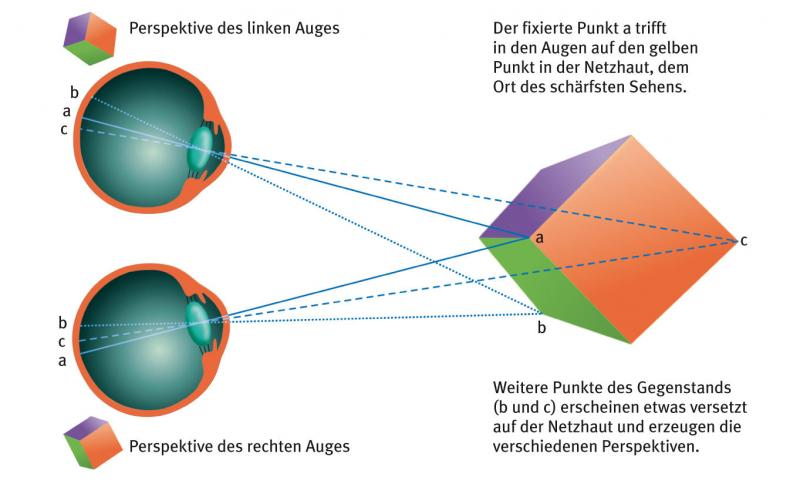
\includegraphics[width=0.45\textwidth]{3D-bild}
   \caption{stereoskopisches Sehen}
   \label{fig:3D}
\end{figure}

Die Bilder des linken und rechten Auges sich an manchen Stellen unterscheiden und menschliches Gehirn kann aus dieser Unterschiede die Positionen, Formen und Großen der Objekte extrahieren.

Damit ein Bild dreidimensional aussieht, ist meistens genug mit approximierten Werten zu arbeiten.
Man nimmt zwei unterschiedliche Bilder, die anhand der mittleren Werte ausgerechnet werden, und zeigt jedem Auge eine davon. 
Damit bekommt man ein 3D-Bild. 
Für manche Anwendungen (wie 3D-Filme, oder stereoskopische Bilder) ist schon genug,  dass ein Bild als 3D interpretiert wird. 
Für uns aber nicht, da mit so eine Realisation unterschiedliche Menschen sehen dasselbe Bild unterschiedlich.
Alle Menschen werden diese Bilder als 3D interpretieren, aber die Position und Größe der gesichteten Objekte können sich stark unterscheiden. Für kritische Anwendung im Fahrzeug, beispielsweise das Anzeigen der Passanten in der realitätserweiternden Sicht mithilfe der Brille, ist dies jedoch entscheidend. Aus dem Grund ist eine individuelle Kalibrierung vorzunehmen.


\subsubsection{Geometrische Beschreibung der Kalibrierung}
Dieses Kapitel beschreibt wofür die Kalibrierung durchgeführt wird und welche Daten dafür benötigt werden.
Die gegebene Daten sind im Abb. \ref{fig:geom} dargestellt. 

\begin{figure}[h]
   \centering
   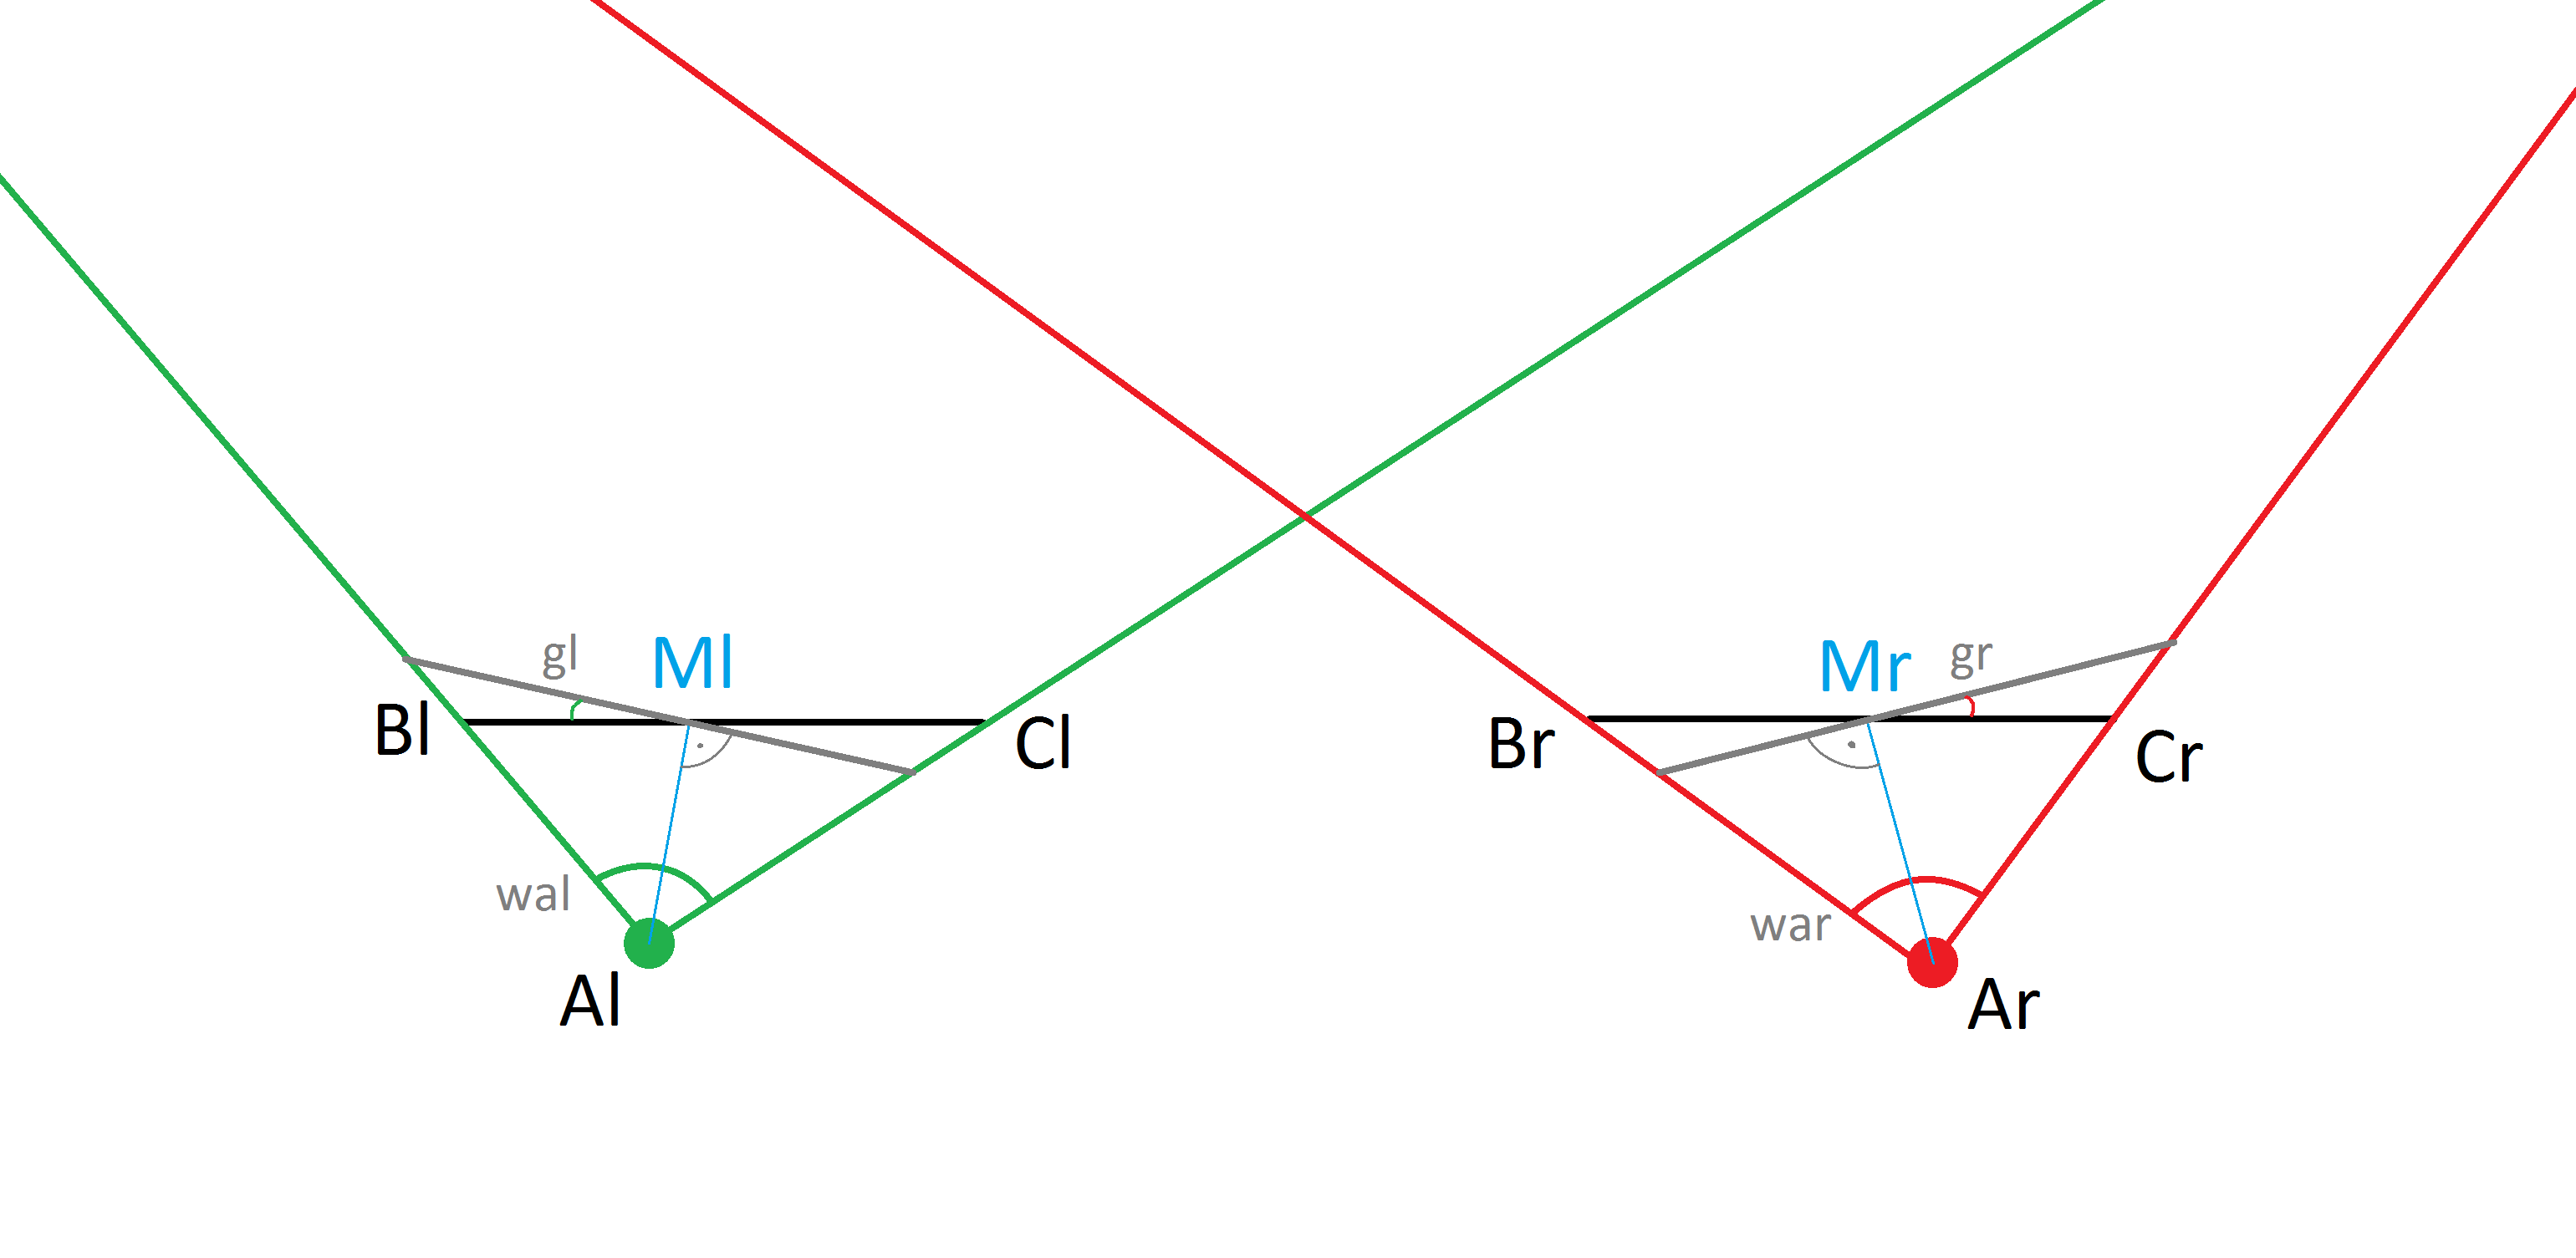
\includegraphics[width=0.45\textwidth]{kalibr-geometrie}
   \caption{Geometrische Beschreibung der Kalibrierung}
   \label{fig:geom}
\end{figure}

Punkte Bl, Cl bzw. Br, Cr sind die Endpunkte des linken bzw. rechten Bildschirms der Brille.
Die Punkte Al (grün) bzw. Ar (rot) beschreiben die Positionen der Augen.
wal bzw. war sind die Sehwinkel des Benutzers durch welche die Bildschirme und dort dargestellte Objekte gesehen werden. 
Blaue Linien ml und mr sind Winkelhalbierenden.

Für die Anzeige der Bilder auf der Brillenbildschirme, werden Augen als Kameras interpretiert und damit werden benötigte Bilder erstellt.
Dementsprechend sind die Winkel wal und war die Öffnungswinkel dieser Kameras.
Wie auf dieser Abb. ref{fig:geom} gut zu sehen ist, müssen die Augenpositionen nicht unbedingt in der Mitte des Bildschirms liegen.
In meisten Anwendungen, die Kameras simulieren, ist aber vorausgesetzt, dass die Kameras in der Mitte sind.
Das ist dasselbe, wie dass der Winkelhalbierende der Öffnungswinkel senkrecht zur Bildschirm ist.
Wir nehmen an, dass dafür benötigte Drehwinkel gl bzw. gr keine entscheidende Rolle in der Bildanzeige spielt.
Mit dieser Annahme rechnen wir die Winkel gl und gr aus  um die virtuellen Kameras theoretisch zu drehen.
Das wird benötigt um passende Daten für die Benutzung anderer Anwendungen zu bekommen.

\subsection{Augensimulierung mithilfe der virtuellen Rviz-Kameras }
Für die technische Realisierung des Stereoskopischen 3D werden alle erkannten Objekte in die virtuelle Welt auf korrespondierende Positionen übertragen. Zusätzlich dazu werden 2 Kameras in der virtuellen Welt definiert, die permanent Sichtbilder auf die virtuellen Objekte ermöglichen. Allerdings reicht eine einfache Augensimulation aufgrund der technischen Voraussetzungen nicht aus. Denn die realen Display ist sind nur ein kleiner integrierter Teil der Brillen und unterscheidet hinsichtlich der Brennweite und des Öffnungs- und Drehwinkels erheblich von den Standardeinstellungen einer virtuellen Kamera ab. Aus diesem Grund sind an den virtuellen Kameras Konfigurationen und Änderungen notwendig, die nun im Weiteren erläutert werden soll. 


\subsubsection{Einstellung des Öffnungswinkels der virtuellen Kameras}

Je nach anatomischen Aufbau des Gesichts hinsichtlich  der Nasenform und der Augenpositionen des menschlichen Nutzers, variiert der tatsächliche Öffnungswinkel, der aufgrund des Abstandes vom Auge zur Brille entsteht. Im Rahmen des Praktikums wurden mithilfe eines eigenständigen Versuches Augenpositionen relativ zur Kamera gemessen. Da die Lage der Brillendisplays zur Kamera als konstant angenommen wird, ist der Abstand zwischen Auge und Brillendisplays nun bestimmbar.

Da der Öffnungswinkel der virtuellen Kameras nicht direkt manipuliert werden kann, wird ein alternativer Weg verwendet. Dabei wurde die virtuelle Kamera mithilfe der intrinsischen Parameter verändert. Zum einen entspricht die Brennweite f der virtuellen Kamera dem Abstand der Augen zum Display, zum anderen bilden die Größen der Brillendisplays die Grundlage für die Berechnung der Auflösung der virtuellen Kameras. Konkrete Berechnung findet sich in der Projektionsmatrix in \ref{table:instrisische Kameraparameter} wieder. $f_x$ und $f_y$ beschreiben die fokalen Längen in Pixel (d.h. Abstand*px/m), $c_x$ und $c_y$ beschreiben den "Principle Point" der Kamera, welche sich aus der Auflösung (1280x 760 für die Vuzix-Brille) ergibt. 

%

\begin{equation}
\begin{pmatrix}
f_x & 0& 0& c_x \\
0 & f_y & 0 & c_y\\ 
0 & 0&   1 & 0  
\end{pmatrix}
\label{table:instrisische Kameraparameter}
\end{equation}

Die Displaygrößen variieren je nach Abstand Auge-Display. Die gemessenen Werte befinden sich mit obengenannten Größen in \ref{table:Messwerte DisplayAuge}.
%
 \begin{table}[ht]

 \begin{tabular}{lc} 
  Beschreibung & Wert \\ \\
  Displaypixelbreite & 2.0403 cm/px \\
  Displaypixellänge &  1.9537 cm/px \\
 \end{tabular}
 \caption{Gemessene Größen für eine Versuchsperson}
 \label{table:Messwerte DisplayAuge}
 \end{table}



%
Mit der kalibrierten Brennweite und dem Blickwinkel der virtuellen Kameras können nun Objekte in der richtigen Größen angezeigt werden, wie sie von den Augen wahrgenommen werden sollen. Allerdings weicht die wahrgenommene Position der Objekte von der realen Position noch stark ab. 

\subsubsection{Drehwinkeleinstellung}
3-D-Sehen wird erst ermöglicht, wenn für beide Augen ein entsprechender Drehwinkel (d.h. Drehung in der horizontalen Ebene) eigestellt werden. Dies wurde im \ref{sec:Stereoskopisches 3D} erläutert.  Entsprechende Drehwinkeln für das linke Auge $gl$ und für das rechte $gr$ werden dabei jeweils für die korrespondierende, virtuelle Kamera verwendet
Es ist dabei eine wichtige Annahme zu berücksichtigen. Im Verhältnis zum Brillendisplay liegen die Augen hinsichtlich der Höhe in der Mitte. Dies bedeutet dass eine Betrachtung der Drehung des Winkels in der vertikalen Ebene ebenfalls notwendig ist. Dies ist in realen Anwendungen nicht zu vernachlässigen und darf auch deshalb in späteren Entwicklungen nicht außer Acht gelassen werden.

Mithilfe obiger Konfigurationen lassen sie sowohl erkannte reale Objekte als auch virtuelle Objekte anzeigen.  Ein Beispiel dafür findet sich in Abbildung \ref{fig:Virtuelle Quadrate aus Prezi}

\begin{figure}[h]
   \centering
   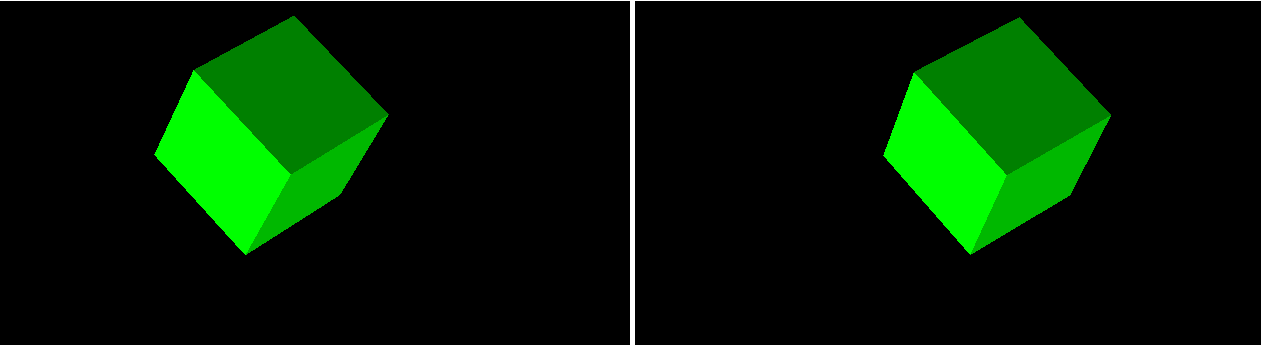
\includegraphics[width=0.45\textwidth]{3d.png}
   \caption{Virtuelle Objekte für das linke und das rechte Auge}
   \label{fig:Virtuelle Quadrate aus Prezi}
\end{figure}

\subsection{Ausblick}
Um die Implementierung einsatztauglich zu machen, müsste für die Kalibrierung die dynamische Einblende der Punkteanzahl ergänzt werden. Während dem Kalibrieren kann die Güte der eingegebenen Punkte festgestellt werden, aus dieser kann abgeleitet werden, wie viele weitere Punkte noch nötig sind. Desweiteren wäre es möglich, dem Benutzer deutlicher zu signalisieren, mit welchem Auger er gerade kalibrieren muss.

Desweiteren wäre eine Plausibilisierung des Ergebnises angebracht, sodass Fehlkalibrierungen direkt erkannt werden können. Hierzu würden Schwellwerte ausreichen.

